\documentclass{article}
\usepackage[utf8]{inputenc}
\usepackage{graphicx}

\title{Lab 4 Redes: "Redes de Datos
Comprobación del funcionamiento del algoritmo STP e
implementación de VLAN
"}
\author{Vicente Lopez\\Esteban León\\Sebastian Antón\\Jorge Ramirez\\Profesor: Jose Alejandro Perez\\Ayudante: Alexis Inzunza}
\date{Mayo 2017}

\usepackage{natbib}
\usepackage{graphicx}

\begin{document}
\begin{figure}[h]

\includegraphics[width=0.45\textwidth]{logo_udp.png}
\maketitle
\end{figure}

\section{Indice}
2 Introducción -------------------------------------------------1\\
3 Actividad 1---------------------------------------------------2\\
4 Actividad 2---------------------------------------------------4\\
5 Conclusión -------------------------------------------------- 6\\
6 Bibliografia -------------------------------------------------- 6\\

\section{Introducción:}
En este laboratorio relizaremos una topologia en cisco packet tracer y la configuraremos para comprobar el funcionamiento del algoritmo STP implementando VLANS.\\\\

\section{Actividad 1:}
Realice la siguiente topologia en cisco packet tracer:\\\\
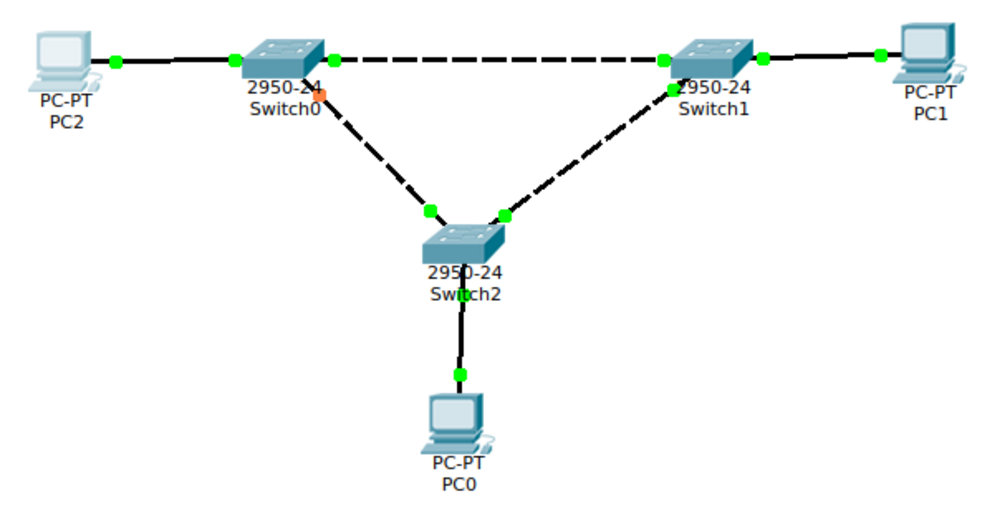
\includegraphics[scale=0.5]{stp.PNG}\\\\
Luego de realizar la anterior topologia, realize las siguientes actividades:\\
Actividad 1-1:\\
Desactive el protocolo STP\\
Actividad 1-2:\\
Active el protocolo STP\\
Actividad 1-2:\\
Configure las prioridades de los switches\\

\subsection{Preguntas Actividad 1:}
a) ¿Qué camino realizara un paquete que para llegar desde el switch 0 hasta el
switch2? Correspondiente a la actividad 1-1\\
b) ¿Qué camino realizara un paquete que para llegar desde el switch 2 hasta el
switch1? Correspondiente a la actividad 1-1\\

Lo siguiente responde a las preguntas “a” y “b”: Como la actividad 1-1 corresponde a la desactivación del protocolo STP de la vlan 1, se genera una "tormenta de broadcast", que es un bucle o ciclo infinito de consultas ARP, por lo que se satura la red.\\\\\\\\\\

c) ¿Qué camino realizara un paquete que para llegar desde el switch 2 hasta el
switch0? Correspondiente a la actividad 1-2\\\\
Un paquete enviado desde el PC0 pasa por el switch2, este realiza una consulta ARP hacia los equipos conectados con los puertos activos, la cual se dirige hacia el switch1. Este switch realiza la misma acción y envía la consulta ARP hacia el PC1 y hacia el switch2, como el paquete no va dirigido hacia el PC1, este rechaza el mensaje. El switch0 realiza la consulta ARP y por el puerto que está conectado al switch0 (fa0/1), no puede enviar, ya que este es un puente alterno. Por el otro puerto (fa0/2) se encuentra al destinatario del paquete y le hace entrega de este. Posterior a esto, PC2 envía un mensaje de vuelta indicando que el paquete fue recibido.\\\\
d) ¿Qué camino realizara un paquete que para llegar desde el switch 1 hasta el
switch0? Correspondiente a la actividad 1-2\\\\
Cuando el PC1 envía un paquete hacia el PC2, lo envía al switch1, este envía consultas ARP hacia el switch2 y hacia el switch0. El switch2 recibe la consulta y replica esta hacia el switch0 y hacia el PC0. Como la conexión entre switch2 y el switch0 es una conexión alterna, no llega el paquete (evitando tormenta de broadcast). El PC0 rechaza el paquete ya que no va dirigido hacia él. El switch0 recibe la consulta ARP y consulta al PC2 si es el destinatario, al ser afirmativa la respuesta, se le entrega el paquete al PC2 y este envía una respuesta hacia el PC1 sobre la recepción del paquete.\\\\


\section{Actividad 2:}
Realice la siguiente topologia en cisco packet tracer:\\
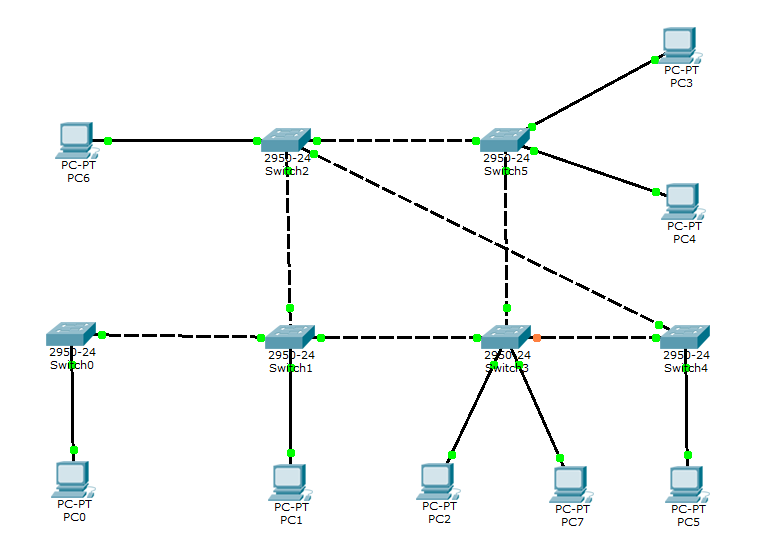
\includegraphics[scale=0.6]{stp2.png}\\\\

Cuando haya terminado con la configuración de los switches, proceda a asignar IP a cada equipo de la
topología. Utilice el segmento 10.0.0.1/24 para configurar los equipos excepto el PC0 que debe utilizar
la IP 10.0.0.8\\

luego de lo realizado anteriormente configure las siguientes VLANS mediante la siguiente tabla.\\

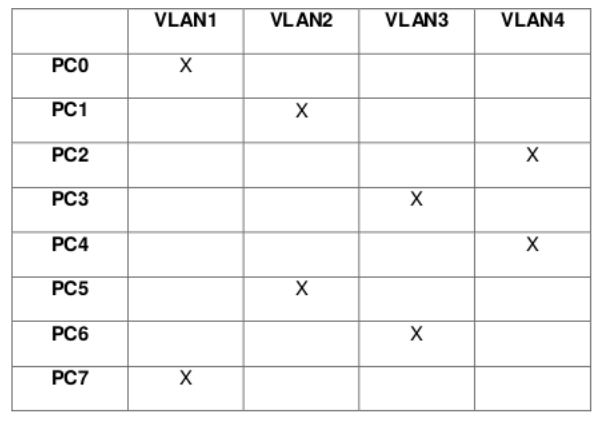
\includegraphics[scale=0.8]{tabla.png}\\

\subsection{Preguntas Actividad 2:}
a) ¿Cuál es la diferencia del modo Access y el modo Trunk en un switch?\\
La diferencia entre el modo Access y el modo Trunk, es que en el Access, se utiliza una sola VLAN, y es para conectar únicamente dispositivos, en cambio el modo Trunk, permite manejar el tráfico de varias VLANS desde un mismo puerto, es decir, nos ahorra tener que conectar otro cable (uno para cada VLAN), de este modo las VLANS se conectan a través del mismo medio físico. Este modo es utilizado cuando queremos conectar equipos de red, como 2 switch.\\\\
b) ¿Qué ocurre si conecto una puerta en modo Trunk a un PC?\\
Realizamos el procedimiento de conectar puerto en modo Trunk a un pc, y lo que ocurrió fue que entre el switch y el PC no establecen conexión. Esto debido a que la conexión Trunk es para la comunicación de manera física entre las vlan entre switches y no en conexión entre switch y PC.\\\\
c) ¿Qué ocurre si conecto dos switches, uno en modo access y otro en modo trunk?\\
 Lo que ocurriría es que como el modo access soporta solo una vlan, mientras que el modo Trunk soporta múltiples vlans, la comunicación sólo podría llevarse a cabo en la vlan a la que está configurado el puerto en modo access (de manera estática), por lo que las demás vlans no podrían pasar entre estos switches.\\
d) ¿Qué camino realizara un paquete que para llegar desde el switch 1 hasta el switch 0?\\
El paquete irá directamente al switch 0 en un paso , debido a que están conectados directamente. \\

\section{Conclusión}
Luego de realizar este laboratorio logramos aprender sobre el algoritmo STP, sabiendo como funciona y lo importante que es para evitar el colapso de una topologia.\\


\section{Bibliografia}
Laboratorio N4:Comprobación del funcionamiento del algoritmo STP e implementación de VLAN.\\
\end{document}